
\subsection{Quirks mode}
Zer gertatuko da DOCTYPE etiketa ez badugu idazten?
Gaur egungo nabigatzaileek \texttt{DOCTYPE switch} izeneko sarrera erabiltzen dute CSS-a nola irudikatu jakin ahal izateko. Bi aukera daude: bateragarritasun modua (\texttt{quirks mode}) eta estandarrak betetze modua (\texttt{strict rendering mode}). Bateragarritasun moduan, nabigatzaileak ez du kontutan izango estandarrak eskatzen dituen hainbat arau (90. hamarkadan horrela funtzionatzen zuten nabigatzaileek). Berriz, estandarrak betetze moduan, nabigatzaileak ahalik eta modu zuzen eta zorrotzenean saiatuko da estandarrak betetzen, nahiz eta jokabide horrek ezusteko emaitzak pantailaratu. Adibidez, demagun horrelako CSS estilo bat zehaztu dugula:

\begin{minipage}{\linewidth}
\begin{lstlisting}
a {
  outline: none;
  text-decoration: none;
  padding: 2px 1px 0;
}

a:link {
  color: FF0000; /* hau akats bat da */
}
\end{lstlisting}
\end{minipage}

Estandarrak betetze moduan koloreak \# aurrizkiaz agertu behar dira. Berriz, bateragarritasun moduan ez da guztiz beharrezkoa.  Hori dela eta bateragarritasun moduan estekak (A etiketak) berdez margotuko dira. Berriz, estandarrak betetze moduan, defektuzko koloreaz (urdinez).

Nola jakin orri baten modua? Iturburu kodea aztertuz edo, Firefox-en bagaude, eskubiko botoia sakatu eta "Orriaren informazioa" aukera hautatuz, "Errendatzeko moduan" fijatuko gara:

\begin{figure}[ht]
	\centering
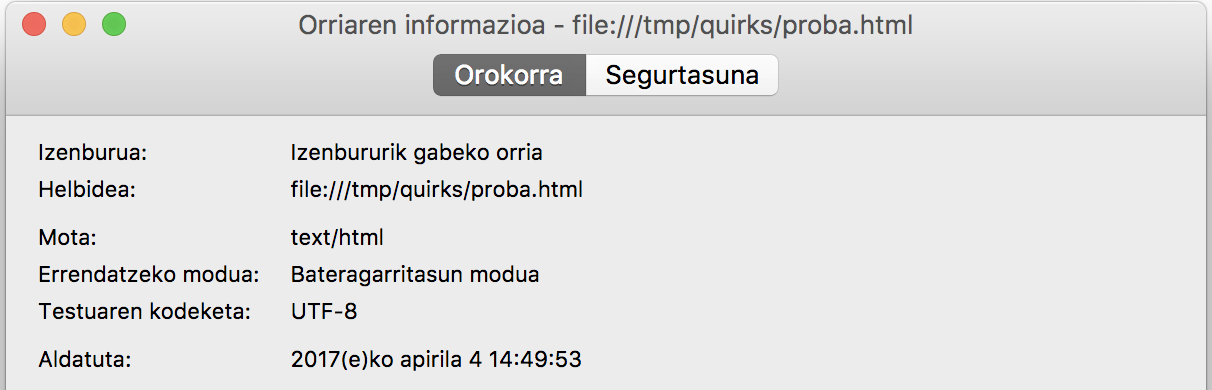
\includegraphics[trim=0cm 1cm 0cm 0cm, clip=true, width=0.5\textwidth]{img/quirks}
\caption{Orriaren informazio kutxan ikus dezakegu orri batek estandarrak betetze modua edo bateragarritasun modua jarraitzen duen}
\label{fig:quirksmode}
\end{figure}

Erreferentziak: 
Zer da quirks mode? http://www.quirksmode.org/css/quirksmode.html
Zein da quirks mode-ren eragina? https://developer.mozilla.org/en-US/docs/Mozilla/Mozilla\_quirks\_mode\_behavior
